\documentclass[preprint,3p,twocolumn]{elsarticle}


\usepackage[x11names,dvipsnames,table]{xcolor} %for use in color links
\usepackage{subfig}
\usepackage{svg}
\usepackage{url}
\usepackage{flushend}
\usepackage{xspace}
\usepackage{enumitem}
\usepackage{hyperref}
\usepackage{multirow}


\newcommand{\todo}[1]{\color{blue}\xspace[\emph{#1}]\xspace\color{black}}
\newcommand{\note}[1]{\color{green}\textbf{Note: }\textit{#1} \color{black}}

\begin{document}

\begin{frontmatter}

%% Title, authors and addresses

%% use the tnoteref command within \title for footnotes;
%% use the tnotetext command for theassociated footnote;
%% use the fnref command within \author or \address for footnotes;
%% use the fntext command for theassociated footnote;
%% use the corref command within \author for corresponding author footnotes;
%% use the cortext command for theassociated footnote;
%% use the ead command for the email address,
%% and the form \ead[url] for the home page:
%% \title{Title\tnoteref{label1}}
%% \tnotetext[label1]{}
%% \author{Name\corref{cor1}\fnref{label2}}
%% \ead{email address}
%% \ead[url]{home page}
%% \fntext[label2]{}
%% \cortext[cor1]{}
%% \address{Address\fnref{label3}}
%% \fntext[label3]{}

\title{Architectures for workflow integration in science gateways}

%% use optional labels to link authors explicitly to addresses:
%% \author[label1,label2]{}
%% \address[label1]{}
%% \address[label2]{}

\author{}

\address{}

\begin{abstract}
%% Text of abstract

\end{abstract}

\begin{keyword}
%% keywords here, in the form: keyword \sep keyword

%% PACS codes here, in the form: \PACS code \sep code

%% MSC codes here, in the form: \MSC code \sep code
%% or \MSC[2008] code \sep code (2000 is the default)

\end{keyword}

\end{frontmatter}

\journal{Future Generation Computer Systems}

\maketitle

\section{Introduction}

\todo{Say that the review is done based on our experience with VIP,
  CBRAIN, and to some extent SHIWA.}

\paragraph{Context} The question of integrating workflow engines in
science gateways can be seen at various levels, corresponding to
various definitions of workflows. One level is the SHIWA level, where
it was considered that workflow engines are aware of the DCI (and 'D'
is important because of data transfers, proxies, etc). Another level
is to remove 'D' from the definition: a workflow engine becomes a
program that submits jobs, potentially only to local clusters. It
opens a whole new class of workflow engines that we used to consider
as "applications". For instance, in neuroinformatics: Nipype, PSOM,
but also FSL through the fslsub tool. A workflow engine is not
supposed to be aware of the science gateway.  A wide-array of workflow
engines are available with specificies coming from the application
domain, available tools, etc Their integration in science gateways
becomes critical. Several of the examples presented in the
paper will be taken from medical image analysis, in particular
neuroimaging.

\paragraph{Goal} this paper reviews and compares the architectures to
integrate workflow engines in science gateways.

\paragraph{Contributions}
\begin{itemize}
\item We evaluate architectures based on our experience with existing systems
\item We propose a new architecture
\end{itemize}

\section{Workflow engines and science gateways}

\subsection{Workflow engines}

In the last decade, the e-Science workflow community has developed
high-level workflow systems to help developers access distributed
infrastructures such as grids and web services, resulting in tools
such as Askalon, Hyperflow, MOTEUR, Pegasus, Swift, Taverna, Triana,
VizTrails, WS-PGRADE/gUSE, etc. Such workflow engines usually describe
applications in a specific language that offers operators for parallel
computing, visual description and edition, links with domain-specific
tool repositories, etc. Descriptions and experiments conducted with
e-Science workflow engines were published in journals such as Future
Generation Computer Systems and conference venues such as
WORKS. 

At the same time, specific toolboxes were emerging in various
scientific domains to facilitate interactions between different
software components. In neuroimaging for instance, tools such as
Nipype, PSOM, SPM and FSL provide abstractions and functions to define
processes that handle the data flow between other processes. Soon,
such tools were interfaced to computing systems, in particular
clusters: they were extended to create cluster tasks, handle their
dependencies, and execute them on clusters. For instance, FSL can
launch tasks on SGE through its \texttt{fsl\_sub} tool, Nipype
\todo{...}, PSOM \todo{...}, and SPM \todo{...}. Although distributed
infrastructures are hardly handled, such domain-specific tools have to
be called workflow engines. They represent a tremendous opportunity
for science gateways to leverage existing tools and
applications. Whether these should be combined with e-Science workflow
engines is an open question.

A workflow engine is defined as a software that submits jobs to a
cluster, grid or cloud. Workflows may be expressed in any language,
including scripts. Several workflow engines may be combined in the
same science gateway. Workflow: a process that submits tasks to the
infrastructure. FSL tools, say Feat, can be considered as workflows
when they are configured to submit tasks to clusters using fslsub. A
workflow consists of activities. We are talking only about concrete
workflows with a configuration (see terstyansky et al 2014 "enabling
scientific workflow sharing...")

  Workflow engine: executes workflows, i.e. process their dependencies
  and create computing tasks. Might transfer data too. A workflow
  engine is not supposed to be aware of the science gateway.

\subsection{Science gateways}

Science Gateway: An ecosystem, usually accessible through a web
  portal, that provides tools to access distributed
  infrastructures. Tools usually help users manage data transfers,
  task execution and authentication on multiple computing and storage
  locations. Examples: CBRAIN, VIP, NSG, etc

Multi-engine, multi-language.


\subsection{Infrastructures}

\todo{Maybe this is not relevant}

The infrastructure consists of the computing and storage resources
involved in the workflow execution, and the software services used to
access these resources. Infrastructures can be servers, clusters,
grids or clouds. Some workflow engines may assume specific
characteristics about the infrastructure, such as the presence of a
shared file system between the computing nodes.

\section{Architectures}

The architectures are diagramed in Figure~\ref{fig:architectures}
using the graphical notations shown in
Figure~\ref{fig:notations}. Architectures are described from their
main software \emph{components} and \emph{interactions}. Software
components include science gateway and infrastructure in all
architectures, and workflow service, workflow pool and agent are
involved in some architectures. The workflow engine itself is
represented by a specific symbol. Software interactions among these
components are described in the next Section. \emph{Abstract}
interactions are specific types of interactions that may be
implemented by various different software interactions. An
architecture that has an abstract interaction is an abstract
architecture. Red color is used to represent the components and
interactions that need to be specifically developed to integrate
workflow engines. Tasks refer to computing tasks that are created by
the workflow engine and executed on the infrastructure. Data
represents any type of file, or database that is involved in the
workflow execution and stored on the infrastructure while the workflow
executes. It does not cover workflow parameters such as strings,
numbers, etc. The reminder of this section describes the different
types of interactions involved in the architectures, and details each
architecture.

%http://ieeexplore.ieee.org/stamp/stamp.jsp?tp=&arnumber=4782949

\begin{figure}
\centering
\def\svgwidth{\columnwidth}
\input{figures/notations.pdf_tex}
\caption{Graphical notations}
\label{fig:notations}
\end{figure}

\begin{figure*}
\centering
\hspace*{0.2\columnwidth}
\subfloat[Tight integration]{
\def\svgwidth{0.6\columnwidth}
\input{figures/tight.pdf_tex}
\label{archi:tight}
}
\hfill
\subfloat[Service invocation]{
\def\svgwidth{0.6\columnwidth}
\input{figures/service.pdf_tex}
\label{archi:service}
\hspace*{0.2\columnwidth}
}\\
\hspace*{0.2\columnwidth}
\subfloat[Sub-tasking]{
\def\svgwidth{0.6\columnwidth}
\input{figures/sub-task.pdf_tex}
\label{archi:sub-task}
}
\hfill
\subfloat[Pool]{
\def\svgwidth{0.6\columnwidth}
\input{figures/agent.pdf_tex}
\label{archi:agent}
\hspace*{0.2\columnwidth}
}\\
\subfloat[Nested workflows. Left: abstract model. Right: instantiation with service invocation.]{
\def\svgwidth{0.9\columnwidth}
\input{figures/nested-1.pdf_tex}
\def\svgwidth{0.9\columnwidth}
\input{figures/nested-2.pdf_tex}
\label{archi:nested}
}\\
\subfloat[Workflow import. Left: abstract model. Right: instantiation with service invocation.]{
\def\svgwidth{0.5\columnwidth}
\input{figures/import-1.pdf_tex}
\hfill
\def\svgwidth{0.5\columnwidth}
\input{figures/import-2.pdf_tex}
\label{archi:import}
}
\caption{Architectures}
\label{fig:architectures}
\end{figure*}

\subsection{Interactions}

The interactions involved in the architectures are described below and
labeled consistently with the notations used on
Figure~\ref{fig:architectures}.

\begin{enumerate}[leftmargin=0cm,itemindent=0.6cm,label=\texttt{(\alph*)}]

\item Workflow integration: consists in adding a new workflow to the
  system so that users can execute it. It is triggered by an
  administrator of the science gateway and it results in an interface,
  for instance a web form, where users can enter the parameters of the
  workflow to be executed. The interaction has two aspects:
  (\texttt{a$_1$}) the programs used in the workflow are installed on
  the infrastructure, which may or may not require administrative
  privileges on the infrastructure; (\texttt{a$_2$}) the workflow has
  to be configured in the science gateway so that it becomes available
  to users. Note that integrating a workflow is not the same process
  as integrating a workflow \emph{engine}.
\item Task control: operations to manage tasks on the infrastructure,
  including: authentication, submission, monitoring, termination,
  deletion, etc. Controlling tasks requires to deal with the
  heterogeneous batch managers and meta-schedulers that might be
  available on the infrastructure. When the infrastructure is a grid
  or a cloud, it is for instance implemented using libraries such as
  SAGA, DRMAA, OCCI and similar initiatives \todo{refs needed}.
\item Data control: operations to manage data on the infrastructure,
  such as: upload, download, deletion, browsing, replication, caching,
  etc. Data movements can be triggered by the user in the science
  gateway (\texttt{$c_1$}), to upload input data or download processed
  data. They can also be performed by the workflow engine
  (\texttt{$c_2$}), to transfer data across the infrastructure. The
  infrastructure might offer various data storage backends with
  heterogeneous interfaces. Tools and services such as
  JSAGA~\cite{reynaud2010uniform} or Data Avenue~\cite{hajnal2014data}
  can be used to homogeneize these interfaces.
\item Workflow control: operations to execute a workflow with an
  engine, including: workflow submission, monitoring, termination,
  etc. Workflow control can be coarse-grained (a.k.a. black box) or
  fine-grained (white box). In a coarse-grained model, workflow
  activities are masked and the user only has a global view of the
  workflow execution. In a fine-grained model, user is exposed to the
  workflow topology, i.e. to the outputs of the individual tasks,
  their statuses and so on. 
\item Sub-task control: operations used by tasks to submit sub-tasks
  on the infrastructure, including: submission, monitoring,
  termination, deletion, etc. Sub-task control is similar to
  interaction \texttt{b}, except that information about the parent
  task which submitted a sub-task is usually available and used for
  additional control. For instance, the parent task may wait for all
  its sub-tasks to finish before finishing, and conversely all the
  sub-tasks may be killed if the parent task is killed.
\item Pool-agent: specific to the architecture described
  in Section~\ref{sec:pool}. This is an interaction used when agents retrieve
  work from a central pool. It covers agent registration and
  de-registration to the pool, protocols to send work from the pool to
  the agent, mechanisms to update work status, and so on. 
\item Workflow conversion: translation from one workflow language to
  another one. This interaction may not be available or implementable
  for every workflow language. It has been developed mostly for
  well-structured and relatively simple workflow language such as between GWorkflowDL
  and Scufl~\cite{OLAB-09} and between the 4 languages that were involved in the
  SHIWA initiative. In SHIWA, workflow conversion is done through an
  intermediate representation, the Interoperable Workflow Intermediate
  Representation~\cite{plankensteiner-montagnat-etal:2011}, which
  allows to convert among $n$ workflow languages using $2n$
  interactions instead of $n^2$.
\end{enumerate}

\todo{In the following sections, for each architecture, add a
  description of a real system that implements it: integrated: ?,
  service: VIP, sub-task: CBRAIN-PSOM, pool: SHIWA pool, nested
  workflow: SHIWA CGI, import: SHIWA FGI}

\subsection{Tight integration}

See Figure~\ref{archi:tight}. The workflow engine is tightly
integrated with the science gateway, which means that it is deployed
on the same machine and potentially shares code, libraries and other
software components with the science gateway. For instance, the
workflow engine might be a portlet in a Liferay portal or a controller
in a Ruby on Rails application. The workflow engine and the science
gateway usually share a database where application, users and other
resources are stored. In this model, task and data control are both
initiated from the science gateway. Interactions \texttt{b} and
\texttt{c$_2$} are initiated from the workflow engine while
\texttt{c$_1$} comes from other parts of the science gateway, for
instance a data management interface. As in any other model, the
installation of new workflows in the science gateway (\texttt{a$_2$})
and infrastructure (\texttt{a$_1$}) is done by an administrator, for
security reasons. This is the model adopted in the Catania Science
Gateway Framework~\cite{Ardizzone2012} (see specific documentation on
workflows\footnote{\url{http://bit.ly/1oQrzvQ}}),
CIPRES~\cite{miller2010creating} and LONI Pipeline
Environment~\cite{dinov2009efficient}.


\subsection{Service invocation}

See Figure~\ref{archi:service}. The workflow engine is available
externally to the science gateway, in a service. The science gateway
controls the service through a specific interaction (\texttt{d}) that
might be implemented as a web-service call (e.g. RESTful or SOAP), as
a command-line or as any other method that offers a well-defined
interface to the workflow engine. The workflow engine might be invoked
either as a black box that completely masks the infrastructure and
workflow activities, or as a white box that allows for some
interaction with them. The workflow engine is responsible for
controlling the tasks on the infrastructure (\texttt{b}) and for
performing the required data transfers to execute them
(\texttt{c$_2$}). User data is usually managed through the science
gateway (\texttt{c$_1$}), although it might as well be delivered by
the workflow engine directly to the user.

This architecture is largely adopted, in systems such as Apache
Airvata~\cite{marru2011apache}, Vine
Toolkit~\cite{DBLP:journals/scpe/SzejnfeldDKKKKLPTWDNW10}, Virtual
Imaging Platform~\cite{GLAT-13}, the WS-PGRADE/gUSE
framework~\cite{Kacsuk2012} and the numerous science gateway instances
that rely on
WS-PGRADE/gUSE~\cite{kacsuk2014science}. Figure~\ref{fig:vip-architecture}
shows the architecture of the Virtual Imaging Platform, where the
MOTEUR workflow engine~\cite{GLAT-08i} is invoked as a service at step
\texttt{3} (interaction \texttt{d} on
Figure~\ref{fig:architectures}). Step \texttt{2} on
Figure~\ref{fig:vip-architecture} corresponds to interaction
\texttt{a$_1$}, and step \texttt{4} maps to interactions \texttt{b}
and \texttt{c$_2$} (in VIP, workflow data transfers are performed by
the tasks and embedded in their descriptions).

\begin{figure*}
\centering
\def\svgwidth{1.5\columnwidth}
\input{figures/VIP.pdf_tex}
\caption{Architecture of the Virtual Imaging Platform that integrates
  the MOTEUR workflow engine through service invocation.}
\label{fig:vip-architecture}
\end{figure*}

\subsection{Sub-tasking}

See Figure~\ref{archi:sub-task}. The workflow engine is a particular
task that can submit sub-tasks to the science gateway through
interaction \texttt{e}. The workflow engine keeps track of the
dependencies between the sub-tasks but their execution is delegated to
the science gateway that executes them on the infrastructure through
interaction \texttt{b}. Although the science gateway has no global
vision of the workflow, it can keep track of the sub-tasks submitted
by a given task, for instance to be able to cancel them when the task
is canceled. The science gateway may also implement mechanisms to
facilitate the handling of task dependencies, for instance basic
dependency lists as available in most batch managers (see for instance
attribute \texttt{depend} of option \texttt{-W} in
Torque\footnote{\url{http://docs.adaptivecomputing.com}}).

The science gateway also transfers both user and workflow data across
the infrastructure, so that interactions \texttt{c$_1$} and
\texttt{c$_2$} are both covered by \texttt{c}. In practice, both
\texttt{c$_1$} and \texttt{c$_2$} can be implemented using the same
pieces of code.

The sub-tasking architecture is implemented in CBRAIN~\cite{SHER-14}
where it is used to integrate the PSOM workflow
engine~\cite{bellec2012pipeline} and the FSL toolkit. The CBRAIN-PSOM
integration~\cite{GLAT-16} is illustrated on
Figure~\ref{fig:cbrain-psom-architecture}. On this Figure, the science
gateway is represented by components \texttt{CBRAIN portal} and
\texttt{CBRAIN execution server} and the infrastructure consists of
\texttt{Storage servers} and \texttt{Computing cluster with shared
  file system}. Interaction \texttt{b} on
Figure~\ref{fig:architectures} is implemented by steps \texttt{4},
\texttt{5}, \texttt{7} and \texttt{8}. Interaction \texttt{c} is
implemented by steps \texttt{3} and \texttt{10}. Interaction
\texttt{e} is implemented by step \texttt{6}. The PSOM workflow engine
adopts a pilot-job architecture~\cite{turilli2015comprehensive} where
the a master coordinates workflow execution by submitting workers
and establishing direct communication channels with them. Note how
this peculiar execution model is totally supported by the sub-tasking
architecture.

The CBRAIN-FSL integration is also remarkable as it allows to leverage
FSL pipelines that are written in a very low-level workflow language
(Linux executables and script) that submits tasks uniformly through a
specific tool called \texttt{fsl\_sub}. To integrate FSL in CBRAIN,
\texttt{fsl\_sub} was modified to implement interaction
\texttt{e}\footnote{See \texttt{fsl\_sub} modified script available at
  \url{https://github.com/aces/cbrain-plugins-neuro}} \todo{Add a
  diagram and maybe a code excerpt to illustrate that.}.

\begin{figure}
\def\svgwidth{\columnwidth}
\input{figures/CBRAIN-PSOM.pdf_tex}
\caption{Architecture of the CBRAIN-PSOM integration that illustrates
  the sub-tasking model (Figure extracted from~\cite{GLAT-16}). 1:
  User sends data and pipeline execution request to storage server(s)
  and CBRAIN portal. 2: CBRAIN portal sends execution request to
  execution server on cluster. 3: Execution server transfers data from
  storage server(s). 4-5: Execution server starts PSOM master via task
  scheduler. 6: PSOM master submits PSOM workers to execution
  server. 7-8: Execution server starts PSOM workers through task
  scheduler. 9: PSOM master and workers execute pipeline. 10.
  Execution server transfers results to storage server(s). \todo{Improve graphics}}
\label{fig:cbrain-psom-architecture}
\end{figure}


\subsection{Pool model}
\label{sec:pool}
See Figure~\ref{archi:agent}. Workflows are submitted by the science
gateway to a pool through interaction \texttt{d}. Agents connect to
the pool asynchronously to retrieve and execute workflows through
interaction \texttt{f}. Agents may be started according to various
policies, for instance to ensure load balancing. Agents may wrap
different types of workflow engines. Workflow engine controls tasks
and data on the infrastructure through interactions \texttt{b} and
\texttt{c$_2$}, science gateway transfers user data through
interaction \texttt{c$_1$}, and administrator installs workflow
dependencies through interaction \texttt{a$_1$}.

The pool model was implemented in the SHIWA pool~\cite{ROGE-13}, see
Figure~\ref{fig:shiwa-pool-architecture}. In Figure
~\ref{fig:shiwa-pool-architecture}, interaction \texttt{d} of
Figure~\ref{archi:agent} is implemented in 3 different types of calls
to the pool: workflow submission (\texttt{1} \& \texttt{2}), workflow
status retrieval (\texttt{a} and \texttt{b}), and workflow retrieval
(\texttt{13} \& \texttt{14}). In Figure
~\ref{fig:shiwa-pool-architecture}, interaction \texttt{f} of
Figure~\ref{archi:agent} is implemented through 2 types of calls:
workflow instance retrieval (\texttt{4}, \texttt{5} and \texttt{6}),
and workflow instance update (\texttt{11} and \texttt{12}). Workflow
instance retrieval is used by the agents to fetch work from the
pool. Workflow instance update is used by the agents to update
workflow statuses. In the SHIWA pool, agents can wrap different types
of workflow engines to execute workflows expressed with different
languages. Calls \texttt{0}, \texttt{7}, \texttt{8} and \texttt{9} are
used by workflow engine plugins to declare their supported language
and launch engines, and by workflow engines to report their status to
the agent. These calls are specific to the SHIWA Pool implementation
of the \texttt{agent} component and therefore have no corresponding
representation in Figure~\ref{archi:agent}.

\begin{figure*}
\centering
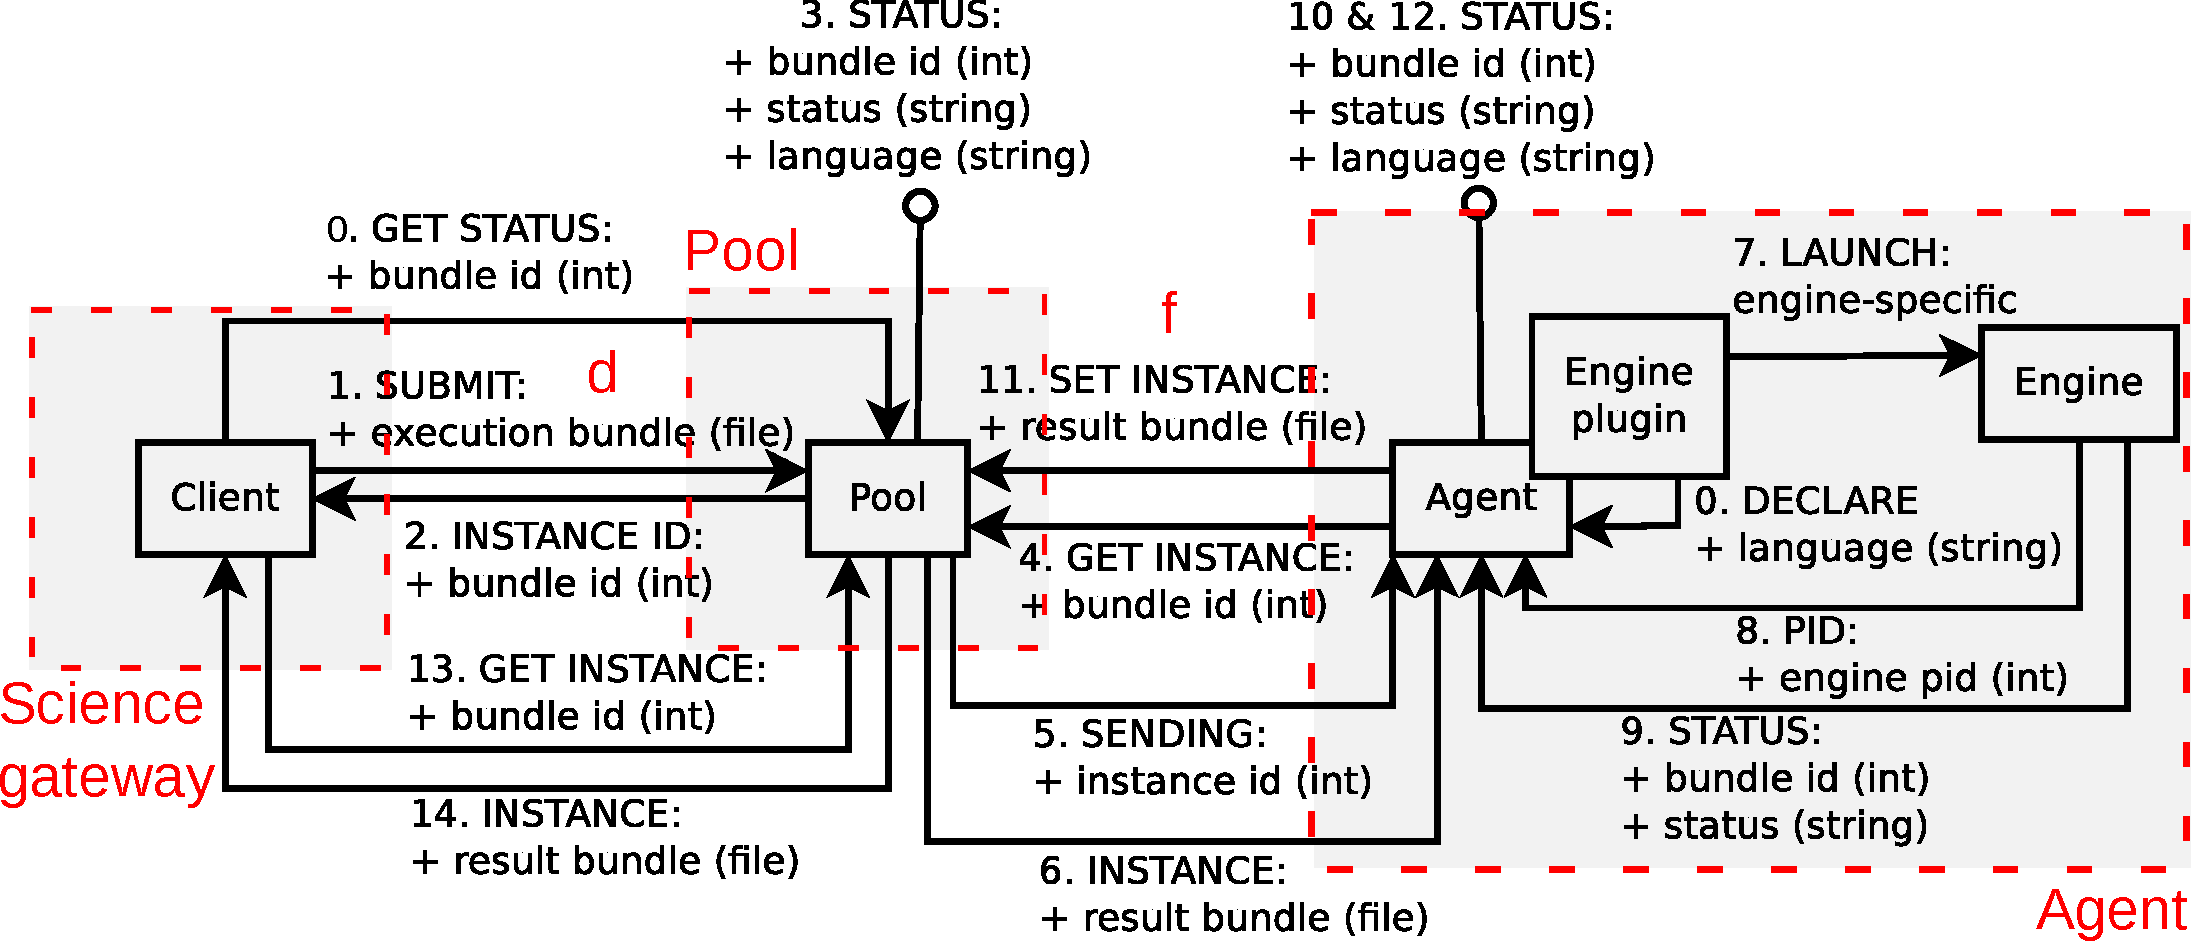
\includegraphics[width=1.5\columnwidth]{figures/pool-interactions.pdf}
\caption{Architecture of the SHIWA pool (Figure reproduced
  from~\cite{ROGE-13}). Circle-terminated arrows indicate messages
  that are broadcast to all pool clients.}
\label{fig:shiwa-pool-architecture}
\end{figure*}


\subsection{Nested workflows}

See Figure~\ref{archi:nested}. In nested workflows (Figure~\ref{archi:nested}-Left), an activity of a
\emph{parent} workflow executed by the \emph{parent} engine is itself
a \emph{child} workflow that is executed by a \emph{child} engine. The
parent and child engines might use different workflow description
languages. They might also execute workflows on different
infrastructures. The parent workflow is also called meta-workflow. The
science gateway communicates with the parent engine through
interaction \texttt{*$_1$}. The science gateway also communicate with
the infrastructure to transfer user data through abstract interactions
\texttt{*$_2$} and \texttt{*$_3$}. Both workflow engines communicate
with the infrastructure through abstract interactions as well,
\texttt{*$_4$} and \texttt{*$_5$}. The parent engine communicates with
the child engine through abstract interaction
\texttt{*$_6$}. Administrator installs workflows in the science
gateway through interaction \texttt{a$_2$}, and installs software on
infrastructures through interactions \texttt{a$_1$}.

Nested workflows are abstract architectural patterns that can be
instantiated in the various architectures described previously. We
focus on instantiation with the service invocation model(see
Figure~\ref{archi:nested}-Right) as this is the most used
architecture. In such an instantiation, we assume that the parent and
child workflow engines are distinct pieces of software that require
different workflow services invoked by distinct \texttt{d}
interactions. If this is not the case, then workflow services can be
collapsed in a single one with a \texttt{d} interaction with
itself. Workflow engines communicate with infrastructures using
\texttt{b} and \texttt{c$_2$}. Science gateway transfer user data to
infrastructures using \texttt{c$_1$} interactions.


Nested workflows have long been available in workflow engines, for
instance in the Taverna workbench~\cite{oinn2004taverna}. They are
also used implicitly in several platforms where workflow engines are
wrapped in workflow activities as any other command-line tool. Nested
workflows were also notably used by the SHIWA Science Gateway to
implement so-called Coarse-Grained workflow
interoperability~\cite{terstyanszky2014enabling}, i.e. to integrate
various workflow engines in a consistent
platform. Figure~\ref{fig:shiwa-architecture} shows the architecture
used in the SHIWA Science Gateway for nested workflow execution with
service invocation as represented in Figure~\ref{archi:nested}. The
parent workflow engine is WS-PGRADE, invoked as a service in the
Science Gateway (step \texttt{1} on
Figure~\ref{fig:shiwa-architecture}, interaction \texttt{d} on
Figure~\ref{archi:nested}). Ten different child engines can be used by
nested workflows, invoked through the \texttt{Submission service}
(step \texttt{2}, interaction \texttt{d}). Each of these engines can
submit jobs and transfer data to a distributed computing
infrastructure (DCI, step \texttt{3}, interactions \texttt{b} and
\texttt{c$_2$}). Data interactions (\texttt{c}) and application
porting ones (\texttt{a}) are not represented on
Figure~\ref{fig:shiwa-architecture}.

\begin{figure*}
\centering
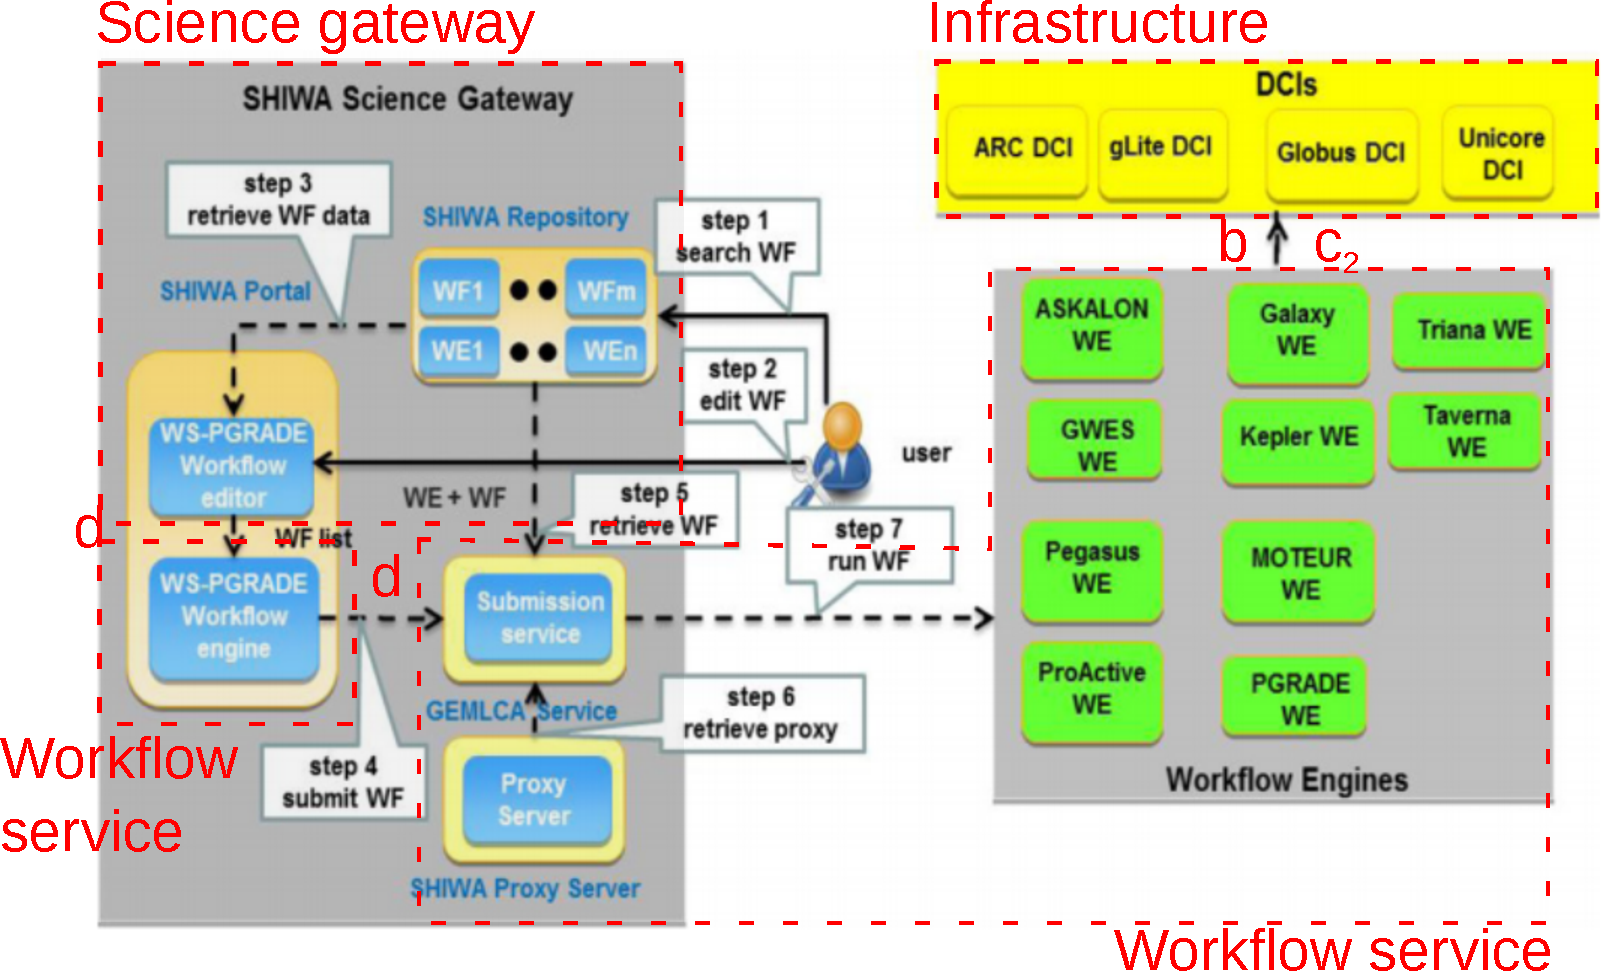
\includegraphics[width=1.5\columnwidth]{figures/shiwa-science-gateway.pdf}
\caption{Nested workflow execution through SHIWA Science Gateway
  (Figure reproduced from~\cite{terstyanszky2014enabling} with
  permission of the first author).}
\label{fig:shiwa-architecture}
\end{figure*}

\subsection{Workflow import}

See Figure~\ref{archi:import}. This is an abstract model that we
instantiate with the service invocation architecture for
consistency. Workflows are integrated in the science gateway through
format conversion from a native format to the science gateway
format. This was implemented in the SHIWA Science Gateway through
the IWIR language that provided a common language for portability
across grid workflow
systems~\cite{plankensteiner-prodan-etal:2013}.

\todo{workflow import is an offline process.}

\section{Evaluation}

See Table~\ref{table:evaluation}. We focus on the integration of
workflow engines in science gateways, i.e. we assume that the science
gateway is already interfaced with the infrastructure.

\subsection{Evaluation metrics}

We use four main criteria to evaluate the architectures: integration
effort, robustness, modularity and scalability. Criteria break down to
specific metrics for which low values indicate good performance.

\todo{Explain these metrics better, including why the related features
  are useful.}

\todo{Refer to the metric codes.}

\emph{Integration} measures the development effort required to build
the architecture, assuming that the science gateway and infrastructure
are already integrated. It is measured by counting on the
architectural diagram the number of interactions and components to
develop or modify. It breaks down to 4 metrics that quantify the
developments related to:
\begin{itemize}[itemsep=0cm]
\item Science gateway (\texttt{I$_1$}),
\item Workflow engine (\texttt{I$_2$}),
\item Infrastructure (\texttt{I$_3$}),
\item Other components (\texttt{I$_4$}).
\end{itemize}
Interactions are counted only once, in the component from which they
originate.


\emph{Robustness} relates to the complexity of the architecture and
its ability to provide relevant debugging information about the
workflow executions. It breaks down to 3 metrics:
\begin{itemize}[itemsep=0cm]
\item Components: number of unique components involved in workflow executions.
\item Interactions: number of unique interactions involved in workflow executions. 
\item Debugging: availability of debugging information about workflow
  activities (1: difficult to obtain; 0: easy to access). Fine-grained
  information about workflow activity is required to properly
  troubleshoot workflow executions.
\end{itemize}

\emph{Modularity} measures the ability to replace elements in the
architecture, or to integrate new elements. Elements include
workflow engines, workflows and infrastructure. It breaks down in 4
metrics:
\begin{itemize}[itemsep=0cm]
\item New engine type: number of interactions or components to modify
  to integrate a new workflow engine type in the
  architecture. Modification of an interaction is deemed necessary
  when the parameters involved in this interaction are
  modified. Modification of a component is required when its code
  needs to be modified or recompiled (science gateway or workflow
  service), or when a new piece of software has to be installed
  (infrastructure only). Adding a new type of workflow engine allows
  to execute the workflows that have been described in the language(s)
  used by the new engine.
\item New engine version: number of interactions or components to
  modify to integrate a new version of a workflow engine in the
  architecture, assuming that another version of the same engine type
  is already available. We assume that different versions of a
  workflow engine share the same interface, i.e. they can be invoked
  using the same software. When this is not the case, the different
  versions have to be considered as different engine types. 
\item New infrastructure: number of interactions or components to
  modify to integrate a new type of infrastructure in the
  architecture.
\item New workflow: number of interactions required to integrate a new
  workflow in the architecture.
\item Meta-workflow: ability to describe meta-workflows from existing
  workflows (1: not available; 0: available).
\end{itemize}

\emph{Scalability} measures the ability of the architecture to support
high workloads. It breaks down into 4 metrics:
\begin{itemize}[itemsep=0cm]
\item New engine instance (0: automated; 1: manual intervention needed; 2: not possible).
\item Elastic engines (0: easy to implement; 1: difficult to
  implement; 2: not available).
\item Distributed engines (0: possible; 1: not possible).
\item Task scheduling (0: difficult; 1: more difficult).
\end{itemize}


%"A Formal Approach to Support Interoperability in Scientific
%Meta-workflows" (reviewed for IWSG and JoGC) has a formal model to
%evaluate CGI and FGI.
%"four major approaches for workflow interoperability include a,b,c,d" (see Terstyanzky et al, "Enabli%ng scientific workflow sharing through CGI...", FGCS 2014) -> read this ref.
% http://www.oreilly.com/programming/free/files/software-architecture-patterns.pdf


\subsection{Tight integration}

\paragraph{Integration} Tightly integrating a workflow engine in a
science gateway requires to modify the science gateway
(\texttt{I$_1$=1}) and to develop interactions \texttt{b}, and
\texttt{c$_2$} in the workflow engine (\texttt{I$_2$=2}). No other
modification is required (\texttt{I$_3$}=\texttt{I$_4$}=0).

\paragraph{Robustness} The science gateway and the infrastructure are
involved in a workflow execution (\texttt{R$_1$}=2), with interactions
\texttt{b}, \texttt{c$_1$} and \texttt{c$_2$}
(\texttt{R$_2$}=3). Debugging is not an issue since the science
gateway can retrieve any information from the workflow engine
directly (\texttt{R$_3$}=0). 

\paragraph{Modularity} Integrating a new type of workflow engine
requires to modify the science gateway as well as interactions
\texttt{b} and \texttt{c$_2$} (\texttt{M$_1$}=3). Updating a workflow
engine version requires modifications in the science gateway
(\texttt{M$_2$}=1). Adding a new infrastructure generates updates in
interactions \texttt{b}, \texttt{c$_1$} and \texttt{c$_2$}
(\texttt{M$_3$}=3). Inserting a new workflow is done through
interaction \texttt{a} (\texttt{M$_4$}=1). Meta-workflows are not
supported by default (\texttt{M$_4$}=1).

\paragraph{Scalability} Adding a new engine instance requires a new
instance of the science gateway, which is in general not possible
since load-balancing mechanisms available in web servers are usually
meant to deal with short web requests rather than long workflow
executions (\texttt{S$_1$}=2). Coherently, elastic engines are usually
not possible either (\texttt{S$_2$}=2).  Distributed engines are not
available by default (\texttt{S$_3$}=1). The scheduling of tasks on
the infrastructure is as complex as in any other architecture since
the workflow engine might implement any kind of scheduling policy
(\texttt{S$_4$}=0).

\subsection{Service invocation} 

\paragraph{Integration} Integrating a workflow engine as a service
requires to develop 3 interactions and 1 component. First, a workflow
service has to be developed and interfaced with the infrastructure
through interactions \texttt{b} and \texttt{c$_2$}
(\texttt{I$_2$}=3). In addtion, the science gateway has to be extended
to call the engine interface \texttt{d} (\texttt{I$_1$}=1).

\paragraph{Robustness} Workflow execution requires 3 components: the
science gateway, the workflow service, and the infrastructure
(\texttt{R$_1$}=3). It involves the 4 interactions \texttt{b},
\texttt{$c_1$}, \texttt{$c_2$} and \texttt{d}
(\texttt{R$_2$}=4). Fine-grained debugging information is usually easy
to obtain since the workflow service provides direct access to the
engine (\texttt{R$_3$}=0).

\paragraph{Modularity} Adding a new type of workflow engine requires
to implement the corresponding workflow service, to modify interaction
\texttt{d}, and to implement interactions \texttt{b} and
\texttt{$c_2$} (\texttt{M$_1$}=4). New engine versions can be added by
updating the workflow service without modifying any interaction
(\texttt{M$_2$}=0). Adding a new type of infrastructure requires
updates in interactions \texttt{b}, \texttt{$c_1$} and \texttt{$c_2$}
(\texttt{M$_3$}=3). New workflows are added in the science gateway or
in the workflow engine through interaction \texttt{a} only
(\texttt{M$_4$}=1). Meta-workflow are not supported by default
(\texttt{M$_5$}=1).

\paragraph{Scalability} The service architecture supports multiple
engine instances through multiple workflow services. In VIP for
instance, this feature has been available from release 1.17 (April
2016). A basic load-balancing mechanism is available that sends new
workflow executions to the engine instance that has the least active
executions. To avoid ``black-hole'' syndromes created by failing
engine instances, engine instances are automatically disabled when
workflows cannot be submitted to them. Adding a new engine instance,
however, requires manual intervention to declare the new instance in
the science gateway (\texttt{S$_1$}=1). Consequently, elastic engines
are difficult to implement because they require a mechanism to update
the science gateway configuration when a new engine instance is
available (\texttt{S$_2$}=1). Distributing the execution of a single
workflow in multiple engines is usually not possible unless the
workflow engine has specific abilities (\texttt{S$_3$}=1). The
scheduling of tasks on the infrastructure is as complex as in any
other architecture since the workflow engine might implement any kind
of scheduling policy (\texttt{S$_4$}=0).

\subsection{Sub-task}

\paragraph{Integration} Integrating a workflow engine as a sub-task
only requires to implement interaction \texttt{e} (\texttt{I$_2$}=1)
and to install the workflow engine on the infrastructure
(\texttt{I$_3$}=1). A new task type is created in the science gateway
only when a new workflow has to be integrated (see M$_4$), but this is
not required to integrate the engine itself (\texttt{I$_1$}=0).

\paragraph{Robustness} Only 2 components and 3 interactions are
involved in workflow execution (\texttt{R$_1$}=2,
\texttt{R$_2$}=3). Obtaining fine-grained information about workflow
activities is not straightforward since the science gateway has no
knowledge about the workflow topology, and the workflow engine is
integrated as a task (\texttt{R$_3$}=1).

\paragraph{Modularity} Integrating a new type of workflow engine
requires to develop interaction \texttt{e} and to install the engine
on the infrastructure (\texttt{M$_1$}=2). Updating an engine version
requires updates only on the infrastructure (\texttt{M$_2$}=1). Adding
a new infrastructure requires to update interactions \texttt{b} and
\texttt{c} in the science gateway (\texttt{M$_3$}=2). New workflows are integrated by
creating a new task in the science gateway through interaction
\texttt{a} (\texttt{M$_4$}=1), and meta-workflows are not available
(\texttt{M$_5$}=1).

\paragraph{Scalability}
New engine instances are spawned and executed on the infrastructure as
any other task upon user submission (\texttt{S$_1$}=0,
\texttt{S$_2$}=0). Such scalability properties are one of the major
interests of the sub-task architecture. Distributed engines are not
supported by default (\texttt{S$_3$}=1). Task scheduling is slightly
more complex than in the other approaches due to the special role of
the task that executes the workflow engine (\texttt{S$_4$}=1). Indeed,
the reliability of this task is critical since all the sub-tasks in
the workflow depend on it and, depending on the recovery capabilities
of the workflow engine, may need to be resubmitted if the workflow
task fails. The workflow task is also longer than all its sub-tasks,
which increases its chances of failure. In addition, task parameters,
for instance estimated walltime, are more difficult to estimate for
the workflow task than for sub-tasks which may generate issues such as
selection of wrong batch queues on clusters. Finally, the
interdependencies between the workflow task and its sub-tasks may
create deadlocks when there is contention. Say for instance that only
1 computing resource is available for the science gateway and that the
workflow task is running on it and submits sub-tasks, then the
sub-tasks could only execute when the resource is available, which
will never happen because the workflow task will not complete until
the sub-tasks complete. This configuration can be generalized to an
infrastructure with $n$ resources where $n$ workflows are
submitted. In practice, however, the number of submitted workflows
usually remains lower than the number of computing resources available
on this infrastructure, which makes such deadlocks unlikely to happen.

\subsection{Pool}

\paragraph{Integration} Integrating workflow engines through the pool
model requires interaction \texttt{d} in the science gateway
(\texttt{I$_1$=1}), interactions \texttt{b} and \texttt{c$_2$} in the
workflow engine (\texttt{I$_2$=2}), the development of the workflow
pool, agent and interaction \texttt{f} between them
(\texttt{I$_4$=3}).

\paragraph{Robustness} The science gateway, workflow pool, agent and
infrastructure are involved in a workflow execution
(\texttt{R$_1$=4}), and these components are connected through 4
interactions (\texttt{R$_2$=4}). Accessing debugging information is
not likely to be an issue since the workflow pool could implement
specific functions for that (\texttt{R$_3$=0}). 

\paragraph{Modularity} Adding a new engine type requires to wrap the
engine in the agent and to update interactions \texttt{b} and
\texttt{c$_2$} (\texttt{M$_1$=3}). Updating the version of an engine
is transparent (\texttt{M$_2$=0}), and integrating a new
infrastructure requires updates in interactions \texttt{b},
\texttt{c$_1$} and \texttt{c$_2$} (\texttt{M$_3$=3}). Integrating a
new workflow is done through interaction \texttt{a} only
(\texttt{M$_4$=1}) and meta-workflows are not available by default
(\texttt{M$_5$=1}).

\paragraph{Scalability} New engine instances only require new agents,
which is easily automated (\texttt{S$_1$=0}) and by design very
suitable for elastic computing (\texttt{S$_2$=0}). For instance,
auto-scaling rules can be implemented to start new agents when the
workload in the science gateway exceeds a certain threshold \todo{ref
  needed}. Distributed engines are not available by default
(\texttt{S$_3$=1}) and task scheduling is as complex as in any other
architecture (\texttt{S$_4$=0}).

\subsection{Nested workflows with service invocation}

\paragraph{Integration} Setting up a nested workflow architecture with
service invocation requires interaction \texttt{d} in the science
gateway (\texttt{I$_1$=1}), and the development of 2 workflow services
with 2 instances of interactions \texttt{b} and \texttt{c$_2$}
(\texttt{I$_2$=5}).

\paragraph{Robustness} Workflow execution involves the science
gateway, 2 workflow services and the infrastructure
(\texttt{R$_1$=4}), which includes 7 interactions
(\texttt{R$_2$=7}). Debugging is difficult because the science gateway
cannot directly access fine-grained information in the sub-workflow
(\texttt{R$_3$=1}).

\paragraph{Modularity} Adding a new type of \emph{parent} engine
requires to implement the corresponding service, to implement
interactions \texttt{b} and \texttt{c$_2$} in the parent engine, and
to implement interaction \texttt{d} in the science gateway and in the
parent service (\texttt{M$_1$=5}). Adding a new type of \emph{child}
engine only requires to implement the corresponding service, to
develop interactions \texttt{b} and \texttt{c$_2$} in the child
engine, and to implement interaction \texttt{d} in the parent service
(\texttt{M$_1$=4}). We use \texttt{M$_1$=4.5} in
Table~\ref{table:evaluation} to reflect both conditions. Adding a new
version in the parent or child engine only requires modifying this
engine (\texttt{M$_2$=0}). Adding a new infrastructure requires to
re-implement interactions \texttt{b} and \texttt{c$_2$} twice, and
interaction \texttt{c$_1$} once (\texttt{M$_3$=5}). Adding a new
workflow is done through interaction \texttt{a}
(\texttt{M$_4$=1}). Meta-workflows are possible, which is one of the
main interest of this architecture (\texttt{M$_5$=0}).

\paragraph{Scalability} As in the service architecture, adding a new
workflow instance requires manual configuration in the science gateway
(instance of a parent engine), or in the parent engine (instance of a
child engine) (\texttt{S$_1$=1}). Similarly, elastic engines are
difficult to achieve (\texttt{S$_2$=1}). Distributed engines are
possible, through meta-workflows (\texttt{S$_3$=0}). Task scheduling
is more complex than in other architectures though, due to the fact
that workflow execution is split in different engines (\texttt{S$_4$=1}).
\subsection{Workflow import with service invocation}

\paragraph{Integration} Compared to the service architecture, workflow
import requires an additional interaction \texttt{g} in the science
gateway (\texttt{I$_1$}=2, \texttt{I$_2$}=3).

\paragraph{Robustness} Since workflow conversion is not involved in
the execution (it is an offline process), metrics are as in the
service architecture (\texttt{R$_1$=3}, \texttt{R$_2$=4},
\texttt{R$_3$=0}).

\paragraph{Modularity} Since adding a new type of workflow engine aims
at supporting more workflows, we consider that it only requires to
re-implement interaction \texttt{g} in this architecture. Note,
however, that implementing interaction \texttt{g} can require very
substantial work depending on the complexity of the language used by
the new engine (\texttt{M$_1$=1}). Based on the same logic, adding a
new engine version only requires modifying interaction \texttt{g}
(\texttt{M$_2$=1}). As in the service architecture, interfacing with a
new infrastructure requires modifications in the workflow service and
in interactions \texttt{b} and \texttt{c$_2$}
(\texttt{M$_3$=3}). Adding a new workflow is done through interactions
\texttt{a} and \texttt{g} (\texttt{M$_4$=2}). Meta-workflows are
available after import, by connecting workflows in the language used
in the science gateway (\texttt{M$_5$=0}).

\paragraph{Scalability}  Since workflow conversion is not involved in
the execution (it is an offline process), metrics are as in the
service architecture (\texttt{S$_1$=1}, \texttt{S$_2$=1},
\texttt{S$_3$=1}, \texttt{S$_4$=0}).

\begin{table*}
\centering
\begin{tabular}{rcccccc}
\textbf{Metric}                      & \textbf{Tight}
                                     & \textbf{Service}
                                     & \textbf{Sub-task}
                                     & \textbf{Pool}
                                     & \textbf{Nested}
                                     & \textbf{Import} \\
\multicolumn{7}{c}{\cellcolor[HTML]{EEEEEE}\textbf{Integration}}\\
Science gateway -- \texttt{I$_1$}    & \cellcolor[HTML]{99FF99}1
                                     & \cellcolor[HTML]{99FF99}1
                                     & \cellcolor[HTML]{99FF99}0  
                                     & \cellcolor[HTML]{99FF99}1
                                     & \cellcolor[HTML]{99FF99}1
                                     & \cellcolor[HTML]{99AA99}2 \\
Workflow engine -- \texttt{I$_2$}    & \cellcolor[HTML]{99AA99}2
                                     & \cellcolor[HTML]{99FF99}3 
                                     & \cellcolor[HTML]{99FF99}1
                                     & \cellcolor[HTML]{99AA99}2
                                     & \cellcolor[HTML]{99AA99}5
                                     & \cellcolor[HTML]{99FF99}3 \\
Infrastructure -- \texttt{I$_3$}   & \cellcolor[HTML]{99FF99}0
                                     & \cellcolor[HTML]{99FF99}0
                                     & \cellcolor[HTML]{99FF99}1
                                     & \cellcolor[HTML]{99AA99}0
                                     & \cellcolor[HTML]{99AA99}0
                                     & \cellcolor[HTML]{99FF99}0 \\
Other -- \texttt{I$_4$}              & \cellcolor[HTML]{99FF99}0
                                     & \cellcolor[HTML]{99FF99}0
                                     & \cellcolor[HTML]{99FF99}0
                                     & \cellcolor[HTML]{99AA99}3
                                     & \cellcolor[HTML]{99AA99}0
                                     & \cellcolor[HTML]{99FF99}0 \\
\textbf{Total}                       & \cellcolor[HTML]{99FF99}\textbf{3}
                                     & \cellcolor[HTML]{99FF99}\textbf{4}
                                     & \cellcolor[HTML]{99FF99}\textbf{2}
                                     & \cellcolor[HTML]{99AA99}\textbf{6}
                                     & \cellcolor[HTML]{99AA99}\textbf{6}
                                     & \cellcolor[HTML]{99AA99}\textbf{5} \\

\multicolumn{7}{c}{\cellcolor[HTML]{EEEEEE}\textbf{Robustness}}\\
Components  --   \texttt{R$_1$}      & \cellcolor[HTML]{99FF99}2
                                     & \cellcolor[HTML]{99DD99}3
                                     & \cellcolor[HTML]{99FF99}2
                                     & \cellcolor[HTML]{99AA99}4  
                                     & \cellcolor[HTML]{99AA99}4 
                                     & \cellcolor[HTML]{99AA99}3 \\
Interactions -- \texttt{R$_2$}       & \cellcolor[HTML]{99FF99}3    
                                     & \cellcolor[HTML]{99DD99}4
                                     & \cellcolor[HTML]{99DD99}3      
                                     & \cellcolor[HTML]{99AA99}4  
                                     & \cellcolor[HTML]{99AA99}7      
                                     & \cellcolor[HTML]{99AA99}4 \\
Debugging --    \texttt{R$_3$}       & \cellcolor[HTML]{99AA99}0          
                                     & \cellcolor[HTML]{99FF99}0
                                     & \cellcolor[HTML]{99AA99}1
                                     & \cellcolor[HTML]{99FF99}0
                                     & \cellcolor[HTML]{99AA99}1
                                     & \cellcolor[HTML]{99FF99}0 \\
\textbf{Total}                       & \cellcolor[HTML]{99FF99}\textbf{5}
                                     & \cellcolor[HTML]{99CC99}\textbf{7}
                                     & \cellcolor[HTML]{99CC99}\textbf{6}
                                     & \cellcolor[HTML]{99BB99}\textbf{8}
                                     & \cellcolor[HTML]{99AA99}\textbf{12}
                                     & \cellcolor[HTML]{99BB99}\textbf{7} \\
\multicolumn{7}{c}{\cellcolor[HTML]{EEEEEE}\textbf{Modularity}}\\
New engine type -- \texttt{M$_1$}    & \cellcolor[HTML]{99AA99}3
                                     & \cellcolor[HTML]{99DD99}4
                                     & \cellcolor[HTML]{99FF99}2
                                     & \cellcolor[HTML]{99DD99}3
                                     & \cellcolor[HTML]{99DD99}4.5
                                     & \cellcolor[HTML]{99AA99}1 \\
New engine version -- \texttt{M$_2$} & \cellcolor[HTML]{99AA99}1
                                     & \cellcolor[HTML]{99FF99}0
                                     & \cellcolor[HTML]{99FF99}1
                                     & \cellcolor[HTML]{99FF99}0
                                     & \cellcolor[HTML]{99FF99}0
                                     & \cellcolor[HTML]{99FF99}1 \\
New infrastructure -- \texttt{M$_3$} & \cellcolor[HTML]{99FF99}3
                                     & \cellcolor[HTML]{99FF99}3
                                     & \cellcolor[HTML]{99FF99}2
                                     & \cellcolor[HTML]{99FF99}3
                                     & \cellcolor[HTML]{99FF99}5
                                     & \cellcolor[HTML]{99FF99}3 \\
New workflow -- \texttt{M$_4$}       & \cellcolor[HTML]{99FF99}1
                                     & \cellcolor[HTML]{99FF99}1
                                     & \cellcolor[HTML]{99FF99}1
                                     & \cellcolor[HTML]{99FF99}1
                                     & \cellcolor[HTML]{99FF99}1
                                     & \cellcolor[HTML]{99AA99}2 \\
Meta-workflow  -- \texttt{M$_5$}     & \cellcolor[HTML]{99AA99}1
                                     & \cellcolor[HTML]{99AA99}1  
                                     & \cellcolor[HTML]{99AA99}1
                                     & \cellcolor[HTML]{99AA99}1
                                     & \cellcolor[HTML]{99FF99}0
                                     & \cellcolor[HTML]{99AA99}0 \\
\textbf{Total}                       & \cellcolor[HTML]{99AA99}\textbf{9}
                                     & \cellcolor[HTML]{99EE99}\textbf{9}
                                     & \cellcolor[HTML]{99FF99}\textbf{7}
                                     & \cellcolor[HTML]{99EE99}\textbf{8}
                                     & \cellcolor[HTML]{99FF99}\textbf{10.5}
                                     & \cellcolor[HTML]{99AA99}\textbf{7} \\
\multicolumn{7}{c}{\cellcolor[HTML]{EEEEEE}\textbf{Scalability}}\\
New engine instance -- \texttt{S$_1$}& \cellcolor[HTML]{99AA99}2
                                     & \cellcolor[HTML]{99AA99}1
                                     & \cellcolor[HTML]{99FF99}0
                                     & \cellcolor[HTML]{99FF99}0
                                     & \cellcolor[HTML]{99AA99}1
                                     & \cellcolor[HTML]{99AA99}1 \\
Elastic engines -- \texttt{S$_2$}    & \cellcolor[HTML]{99AA99}2
                                     & \cellcolor[HTML]{99DD99}1
                                     & \cellcolor[HTML]{99FF99}0
                                     & \cellcolor[HTML]{99FF99}0
                                     & \cellcolor[HTML]{99DD99}1
                                     & \cellcolor[HTML]{99DD99}1 \\
Distributed engines -- \texttt{S$_3$}& \cellcolor[HTML]{99AA99}1
                                     & \cellcolor[HTML]{99AA99}1
                                     & \cellcolor[HTML]{99AA99}1
                                     & \cellcolor[HTML]{99AA99}1
                                     & \cellcolor[HTML]{99FF99}0
                                     & \cellcolor[HTML]{99AA99}1 \\
Task scheduling -- \texttt{S$_4$}    & \cellcolor[HTML]{99FF99}0
                                     & \cellcolor[HTML]{99FF99}0
                                     & \cellcolor[HTML]{99AA99}1
                                     & \cellcolor[HTML]{99FF99}0
                                     & \cellcolor[HTML]{99FF99}1
                                     & \cellcolor[HTML]{99FF99}0 \\
\textbf{Total}                       & \cellcolor[HTML]{99AA99}\textbf{5}
                                     & \cellcolor[HTML]{99BB99}\textbf{3}
                                     & \cellcolor[HTML]{99DD99}\textbf{2}
                                     & \cellcolor[HTML]{99FF99}\textbf{1}
                                     & \cellcolor[HTML]{99DD99}\textbf{3}
                                     & \cellcolor[HTML]{99BB99}\textbf{3} \\
\multicolumn{7}{c}{\cellcolor[HTML]{EEEEEE}\textbf{Grand total}}\\
                                     & \cellcolor[HTML]{99CC99}\textbf{22}
                                     & \cellcolor[HTML]{99BB99}\textbf{23}
                                     & \cellcolor[HTML]{99FF99}\textbf{17}
                                     & \cellcolor[HTML]{99CC99}\textbf{23}
                                     & \cellcolor[HTML]{99DD99}\textbf{31.5}
                                     & \cellcolor[HTML]{99AA99}\textbf{22}
\end{tabular}
\caption{Architecture evaluation. Lower values (brighter colors) indicate better performance. \todo{update colors and find a more relevant way to compute a grand total without favoring criteria that have more metrics than the others (e.g. normalize each criterion between 0 and 1). Same comment for each sub-total. M1 might be the same as integration. Update nested workflow as infrastructures were separated.}}
\label{table:evaluation}
\end{table*}



\section{Discussion}

Comparison between architectures, per criterion (robustness, etc).

This ignores pre-existing work (e.g. a workflow engine is already available as a service). Migration across architectures too.

These architectures can be combined (give examples). 

The difficulty of implementing interaction g is not properly
reflected. For instance, fsl uses bash, which would be very difficult to convert.

\section{Conclusion}

\section{Acknowledgments}

\todo{FLI-IAM, Labex PRIMES, Ludmer Centre, whatever grant is funding
  POQ for integrating CBRAIN with PSOM.}

We warmly thank Rafael Ferreira da Silva for implementing the VIP
platform and creating Figure~\ref{fig:vip-architecture}.

\section*{References}

\todo{Review use of capitals in references}
\bibliographystyle{elsarticle-num} 
\bibliography{biblio}

\end{document}
\endinput
